%Version 2.1 April 2023
% See section 11 of the User Manual for version history
%
%%%%%%%%%%%%%%%%%%%%%%%%%%%%%%%%%%%%%%%%%%%%%%%%%%%%%%%%%%%%%%%%%%%%%%
%%                                                                 %%
%% Please do NOT use \input{...} to include other tex files.       %%
%% Submit your LaTeX manuscript as one .tex document.              %%
%%                                                                 %%
%% All additional figures and files should be attached             %%
%% separately and NOT embedded in the \TeX\ document itself.       %%
%%                                                                 %%
%%%%%%%%%%%%%%%%%%%%%%%%%%%%%%%%%%%%%%%%%%%%%%%%%%%%%%%%%%%%%%%%%%%%%

%%\documentclass[referee,sn-basic]{sn-jnl}% referee option is meant for double line spacing

%%=======================================================%%
%% to print line numbers in the margin use lineno option %%
%%=======================================================%%

%%\documentclass[lineno,sn-basic]{sn-jnl}% Basic Springer Nature Reference Style/Chemistry Reference Style

%%======================================================%%
%% to compile with pdflatex/xelatex use pdflatex option %%
%%======================================================%%

%%\documentclass[pdflatex,sn-basic]{sn-jnl}% Basic Springer Nature Reference Style/Chemistry Reference Style


%%Note: the following reference styles support Namedate and Numbered referencing. By default the style follows the most common style. To switch between the options you can add or remove “Numbered” in the optional parenthesis. 
%%The option is available for: sn-basic.bst, sn-vancouver.bst, sn-chicago.bst, sn-mathphys.bst. %  
 
%%\documentclass[sn-nature]{sn-jnl}% Style for submissions to Nature Portfolio journals
%%\documentclass[sn-basic]{sn-jnl}% Basic Springer Nature Reference Style/Chemistry Reference Style
\documentclass[sn-mathphys,Numbered]{sn-jnl}% Math and Physical Sciences Reference Style
%%\documentclass[sn-aps]{sn-jnl}% American Physical Society (APS) Reference Style
%%\documentclass[sn-vancouver,Numbered]{sn-jnl}% Vancouver Reference Style
%%\documentclass[sn-apa]{sn-jnl}% APA Reference Style 
%%\documentclass[sn-chicago]{sn-jnl}% Chicago-based Humanities Reference Style
%%\documentclass[default]{sn-jnl}% Default
%%\documentclass[default,iicol]{sn-jnl}% Default with double column layout

%%%% Standard Packages
%%<additional latex packages if required can be included here>
%\usepackage[]{caption}
%\captionsetup[figure]{font=small,skip=0pt}
\usepackage{graphicx}%
\usepackage{multirow}%
\usepackage{amsmath,amssymb,amsfonts}%
\usepackage{amsthm}%
\usepackage{mathrsfs}%
\usepackage[title]{appendix}%
\usepackage{xcolor}%
\usepackage{textcomp}%
\usepackage{manyfoot}%
\usepackage{booktabs}%
\usepackage{algorithm}%
\usepackage{algorithmicx}%
\usepackage{algpseudocode}%
\usepackage{listings}%
%%%%


%\usepackage{algorithm}
%\usepackage{algorithmic}

\usepackage{pdfpages}
\usepackage{tikz}
%\newcommand{\theHalgorithm}{\arabic{algorithm}}
\newcommand{\argmax}{\operatornamewithlimits{argmax}}
\newcommand{\argmin}{\operatornamewithlimits{argmin}}
\def\dd{\,\mathrm{d}}	
\newcommand{\indep}{\perp \!\!\! \perp}
\newcommand{\dep}{\not \!\perp\!\!\!\perp}
\usepackage{amsmath}
\usepackage{amssymb}
\usepackage{mathtools}
%%%%%=============================================================================%%%%
%%%%  Remarks: This template is provided to aid authors with the preparation
%%%%  of original research articles intended for submission to journals published 
%%%%  by Springer Nature. The guidance has been prepared in partnership with 
%%%%  production teams to conform to Springer Nature technical requirements. 
%%%%  Editorial and presentation requirements differ among journal portfolios and 
%%%%  research disciplines. You may find sections in this template are irrelevant 
%%%%  to your work and are empowered to omit any such section if allowed by the 
%%%%  journal you intend to submit to. The submission guidelines and policies 
%%%%  of the journal take precedence. A detailed User Manual is available in the 
%%%%  template package for technical guidance.
%%%%%=============================================================================%%%%

%\jyear{2021}%

%% as per the requirement new theorem styles can be included as shown below
\theoremstyle{thmstyleone}%
\newtheorem{theorem}{Theorem}%  meant for continuous numbers
%%\newtheorem{theorem}{Theorem}[section]% meant for sectionwise numbers
%% optional argument [theorem] produces theorem numbering sequence instead of independent numbers for Proposition
\newtheorem{proposition}[theorem]{Proposition}% 
%%\newtheorem{proposition}{Proposition}% to get separate numbers for theorem and proposition etc.

\theoremstyle{thmstyletwo}%
\newtheorem{example}{Example}%
\newtheorem{remark}{Remark}%

\theoremstyle{thmstylethree}%
\newtheorem{definition}{Definition}%

\raggedbottom
%%\unnumbered% uncomment this for unnumbered level heads



\begin{document}

\title[Feature Importance Depends on Properties of the Data]{Feature Importance Depends on Properties of the Data: Towards Choosing the Correct Explanations for Your Data and Decision Trees based Models}

%%=============================================================%%
%% Prefix	-> \pfx{Dr}
%% GivenName	-> \fnm{Joergen W.}
%% Particle	-> \spfx{van der} -> surname prefix
%% FamilyName	-> \sur{Ploeg}
%% Suffix	-> \sfx{IV}
%% NatureName	-> \tanm{Poet Laureate} -> Title after name
%% Degrees	-> \dgr{MSc, PhD}
%% \author*[1,2]{\pfx{Dr} \fnm{Joergen W.} \spfx{van der} \sur{Ploeg} \sfx{IV} \tanm{Poet Laureate} 
%%                 \dgr{MSc, PhD}}\email{iauthor@gmail.com}
%%=============================================================%%
%\author*[1]{\fnm{First} \sur{Author}}\email{iauthor@gmail.com}

%\affil*[1]{\orgdiv{Department}, \orgname{Organization}, \orgaddress{\street{Street}, \city{City}, \postcode{100190}, \state{State}, \country{Country}}}
\author*[1,2]{\fnm{Célia Wafa} \sur{AYAD}}\email{wafa.ayad@polytechnique.edu}

\author[2]{\fnm{Thomas} \sur{Bonnier}}\email{thomas.bonnier@socgen.com}
%\equalcont{These authors contributed equally to this work.}

\author[2]{\fnm{Benjamin} \sur{Bosch}}\email{benjamin.bosch@socgen.com}

\author[3]{\fnm{Sonali} \sur{Parbhoo}}\email{s.parbhoo@imperial.ac.uk}
\author[1]{\fnm{Jesse} \sur{Read}}\email{jesse.read@polytechnique.edu}

\affil*[1]{\orgdiv{LIX}, \orgname{Ecole polytechnique, IP Paris}, \orgaddress{ \state{Palaiseau}, \country{France}}}

\affil[2]{\orgdiv{MRM}, \orgname{Société Générale}, \orgaddress{\state{Paris}, \country{France}}}

\affil[3]{\orgdiv{Department of Engineering}, \orgname{Imperial College London}, \orgaddress{\state{London}, \country{UK}}}

%%==================================%%
%% sample for unstructured abstract %%
%%==================================%%

\abstract{In order to ensure the reliability of the explanations of machine learning models, it is crucial to establish their advantages and limits and in which case each of these methods outperform. However, the current understanding of when and how each method of explanation can be used is insufficient. To fill this gap, we perform a comprehensive empirical evaluation by synthesizing multiple datasets with the desired properties.
Our main objective is to assess the quality of feature importance estimates provided by local explanation methods, which are used to explain predictions made by decision tree-based models. By analyzing the results obtained from synthetic datasets as well as publicly available binary classification datasets, we observe notable disparities in the magnitude and sign of the feature importance estimates generated by these methods. Moreover, we find that these estimates are sensitive to specific properties present in the data.
Although some model hyper-parameters do not significantly influence feature importance assignment, it is important to recognize that each method of explanation has limitations in specific contexts. Our assessment highlights these limitations and provides valuable insight into the suitability and reliability of different explanatory methods in various scenarios.}

%%================================%%
%% Sample for structured abstract %%
%%================================%%

% \abstract{\textbf{Purpose:} The abstract serves both as a general introduction to the topic and as a brief, non-technical summary of the main results and their implications. The abstract must not include subheadings (unless expressly permitted in the journal's Instructions to Authors), equations or citations. As a guide the abstract should not exceed 200 words. Most journals do not set a hard limit however authors are advised to check the author instructions for the journal they are submitting to.
% 
% \textbf{Methods:} The abstract serves both as a general introduction to the topic and as a brief, non-technical summary of the main results and their implications. The abstract must not include subheadings (unless expressly permitted in the journal's Instructions to Authors), equations or citations. As a guide the abstract should not exceed 200 words. Most journals do not set a hard limit however authors are advised to check the author instructions for the journal they are submitting to.
% 
% \textbf{Results:} The abstract serves both as a general introduction to the topic and as a brief, non-technical summary of the main results and their implications. The abstract must not include subheadings (unless expressly permitted in the journal's Instructions to Authors), equations or citations. As a guide the abstract should not exceed 200 words. Most journals do not set a hard limit however authors are advised to check the author instructions for the journal they are submitting to.
% 
% \textbf{Conclusion:} The abstract serves both as a general introduction to the topic and as a brief, non-technical summary of the main results and their implications. The abstract must not include subheadings (unless expressly permitted in the journal's Instructions to Authors), equations or citations. As a guide the abstract should not exceed 200 words. Most journals do not set a hard limit, however authors are advised to check the author instructions for the journal they are submitting to.}

\keywords{Explainability, Decision Tree Models, Feature Importance, Synthetic Data Generation}

%%\pacs[JEL Classification]{D8, H51}

%%\pacs[MSC Classification]{35A01, 65L10, 65L12, 65L20, 65L70}

\maketitle



\section{Introduction}
Decision tree-based models such as random forest \cite{breimanRandomForests2001a} are widely used machine learning algorithms in data science. Although deep learning has been increasingly popular, especially in domains such as computer vision and natural language processing, random forest, for example, continues to be a competitive option in many types of tabular data in a diverse number of domains, including biology \cite{Multitree} and medicine \cite{ricordeauApplicationRandomForests2010}, where interpretation is paramount. 
Small decision trees operating on understandable feature spaces are naturally interpretable, and although this interpretability is diluted across a large forest, it can be recovered in terms of feature importance, which is a major tool that can be used in practical applications for data understanding, model improvement, or model explainability. 
% Problem 
However, practitioners may lose trust in the importance scores provided for random forest \cite{stroblBiasRandomForest2007}, or simply be unable to use them to answer their research questions from the feature importance result due to a number of reasons \cite{BewareDefaultRandom,LimitationsInterpretableMachine}, for example:
(1) a relative lack of training examples leads to instability where the importance scores change due to only minor changes or additions to the dataset or hyperparameters. (2) Even with a large training set, multiple (possibly equivalent) feature scores can be presented. (3) the feature importance scoring mechanism is thrown off by particular properties of the data distribution such as noise, imbalance, and feature type (in particular, the importance of continuous features is often overestimated).
(4) results where the importance of the feature is assigned to spurious or even random features.  
Practitioners are thus often right to be reluctant to draw conclusions from or place trust in off-the-shelf feature-importance scorers, and we aim to remedy this to some extent with a benchmarking study. 

% Prior work
To remedy this, researchers proposed explainability methods such as \textsf{LIME} \cite{ribeiroWhyShouldTrust2016} and \textsf{SHAP} \cite{lundbergUnifiedApproachInterpreting2017} to explain black-box models by attributing feature importance estimates as explanations of the model's predictions. 
While prior research 
\cite{krishnaDisagreementProblemExplainable2022,attanasioFerretFrameworkBenchmarking2022,camburuCanTrustExplainer2019,bodriaBenchmarkingSurveyExplanation2021,neelyOrderCourtExplainable2021} has already taken the first steps towards analyzing the disagreement of explanation methods for models such as deep neural networks, analyzing the behavior of the wide range of existing explanation methods for random forest or in general ensemble trees still insufficiently explored, with regard to particular data properties and model parameters \cite{flora2022comparing}.

% What we do
Compared to other work, we study the explainability methods suited to explain decision tree-based models. Some of these methods are specific to tree ensembles and the rest are general model-agnostic (which, thus, can also be applied to random forest). We do so with extensive experiments on synthetic alongside real-world datasets, and certain manipulations thereof, which we carry out to isolate and identify aspects which lead to particular results insofar as feature importance. This provides a more thorough understanding, which we use to highlight some limitations of existing methods, and formulate a number of recommendations for practitioners. 
The contribution in this paper is twofold. 
%\textcolor{red}{add that you do compare explanations of the generation model and to ground truth}
% Limitations
%Aside from our focus on random forest, we conduct our study specific to post-hoc feature importance methods, and in the context of binary classification. We also choose the most intuitive aggregation method of local importance, restrict our choice to ten explainability methods and on tabular data.
%impact de la solution
%Our work intends to help understand the strengths and limitations of each method on different data properties and illustrate which method is more relevant to explain which data.
%\textcolor{red}{Our work makes the following contributions:} 
\begin{itemize}
    %\item We isolate data properties in terms of feature interactions (such as feature dependence), type (discrete and continuous), distributions (Gaussian and mixture of Gaussians), noise, irrelevant random variables and class imbalance; that can affect the attribution of feature importance scores
    %\item We introduce a benchmarking framework to efficiently evaluate post-hoc explanation methods designed to explain the predictions of decision tree based models. 
    %\item Our contribution involves the comprehensive assessment of multiple explainability methods concerning their performance relative to specific data properties, including noise levels, feature correlations, and class imbalance. Through this analysis, we aim to delineate the conditions under which each explanation method excels, providing valuable insights into their efficacy and applicability in real-world scenarios.
    %\item We release synthetic datasets on isolated data properties in terms of feature correlation, noise, irrelevant random variables and class imbalance; that can affect the attribution of feature importance scores.
    %\item We leverage recommendations on which explainability method is best suited for which data property by measuring the accuracy of the generated explanations compared to the ground truth feature importance and which of these methods satisfies explanation properties such as the local stability, compactness, consistency and faithfulness.
    %\item We demonstrate on synthetic and real-world datasets the advantages and limitations of the selected explainability methods on the previous properties using the metrics reflecting the desired properties of an explanation. %{\color{red}The code is publicly available at ... ?}
    %\item We also release these synthetic datasets that can be used for other comparison studies. 
    \item Conduct a thorough evaluation of various explainability methods in the context of specific data properties, such as noise levels, feature correlations, and class imbalance, elucidating their strengths and limitations.
    \item Providing valuable guidance for practitioners and researchers on selecting the most suitable explainability method based on the characteristics of their dataset.
    
\end{itemize}

%We propose a framework for benchmarking the feature importance scores attributed by the local and global explainability methods. We do so by: (1) elaborating on the decrease in the model's accuracy on the test set after removing important features and model retraining using the paradigm known as ROAR \cite{hookerBenchmarkInterpretabilityMethods2018} on a variety of datasets including Adult, German Credit Risk, \textsc{Cervical Cancer}, and Heart Disease, (2) assessing the sensitivity of these methods to different hyper-parameters of the random forest model, such as the minimum of samples per leaf used for the inference and the maximum number of the features used during the splits, and (3) carrying out analysis on the local stability of  \textsf{SHAP} \cite{lundbergUnifiedApproachInterpreting2017}, \textsf{LIME} \cite{ribeiroWhyShouldTrust2016}, Local surrogates, and Tree Interpreter \cite{treeinterpreter}. In addition, we measure the covariate shift in the test set by quantifying the sensitivity of these methods to noise and irrelevant variables. 

%Results
%Our results demonstrate that the explanations given by the ten methods do not only disagree, but also are very sensitive to specific data properties.
%We recommend using each of these methods with care to class imbalance, noise, and irrelevant features in addition to the feature distributions and interactions. For example, \textsf{LIME} should be used in cases with less noise and for data with irrelevant variables.
%FIRF and \textsf{TI} on the other hand can be employed for datasets where there is no mixture of continuous and discrete features as they both overestimate the importance of continuous over discrete features. Also, FIPDP and Morris sensitivity can be employed in settings where the features are equally contributors to the prediction making and  \textsf{SHAP} explainers to explain datasets where there are only direct feature contributions because they tend to ignore the indirect effects of some features on the prediction. Lastly, \textsf{LSurro} can be used in datasets with less class imbalance and without random irrelevant variables.
\section{Background}
\paragraph{Post-hoc local explanations for tree based models}\label{meths}
%Explainability methods based on feature importance generation can be categorized to local and global scorers of feature importance. The first explains the individual predictions around a single instance, thus determining which features are important for the prediction attributed to that instance.
%The second visualizes on average which characteristics the model relies on to estimate its outputs.
%Both approaches are important for understanding existing machine learning models. These methods can be categorized into model-agnostic such as Kernel  \textsf{SHAP} \cite{lundbergUnifiedApproachInterpreting2017} or model-specific such as Tree  \textsf{SHAP} \cite{lundbergConsistentIndividualizedFeature2019a} and Tree Interpreter. 
%The evaluation of these methods can be done using subjective (given by domain experts) or objective (such as local stability and consistency) metrics. We discuss some of these metrics in Section \ref{metrics}.
\begin{table}
%\begin{tiny}
\centering
% \resizebox{\textwidth}{!}{
	\begin{tabular}{|l|l|}
		\hline
		 Acronym  & Method\\
		\hline
		 %FIRF &  Feature importance provided by random forest classifier \\
          %PFI & Permutation feature importance \\
           %FIPDP & Importance derived from Partial Dependence Plots (PDP)\\
           \textsf{LSurro} & Local surrogates \cite{molnar2022} \\
           \textsf{LIME} & Local surrogate models \cite{ribeiroWhyShouldTrust2016}\\
           %Morris & Morris sensitivity\\
           \textsf{Kshap} &  Kernel  \textsf{SHAP} \cite{lundbergUnifiedApproachInterpreting2017}\\
           Sshap&  Sampling  \textsf{SHAP} \cite{lundbergUnifiedApproachInterpreting2017}\\
           \textsf{Tshap} & Tree  \textsf{SHAP} \cite{lundbergConsistentIndividualizedFeature2019a}\\
           \textsf{TI} & Tree Interpreter \cite{treeinterpreter}\\
		 \hline
	\end{tabular}
% }
 \caption{\label{tab:accr} Explainability methods under consideration.}
% \end{tiny}
\end{table}
Post-hoc explanation methods can be classified based on explanation scope (global vs. local), model architecture (specific vs. agnostic) and basic unit of explanation (feature importance vs. rule-based). This paper focuses on local post-hoc explanation methods based on feature importance. It analyzes four model agnostic methods in Table \ref{tab:accr} (LIME, \textsf{LSurro}, \textsf{Kshap} and Sshap) and two tree-specific methods (\textsf{Tshap} and TI).

LIME, \textsf{LSurro}, \textsf{Kshap} and \textsf{Sshap} construct local interpretable models such as a linear regression in the neighborhood of the instance that is being explained. These methods differ in the kernel used for the generation of the local neighborhood and the objective that is being optimized. For example, \textsf{LIME} uses an exponential kernel while  \textsf{SHAP} explainers use Shapley kernel, and both use the squared error to minimize the loss between the black box model and the surrogate model.
On the other hand, \textsf{Tshap} and \textsf{TI} both are designed to explain tree based methods such as random forest. \textsf{Tshap} computes the Shapley value for each node in the tree based on the decision splits. While \textsf{TI} decomposes the prediction into the sum of feature contributions and the bias, i.e; the mean given by the root of the decision tree that covers the entire training set.
 %http://blog.datadive.net/interpreting-random-forests/

%In addition to Kernel SHAP, Tree  \textsf{SHAP} and Tree Interpreter, we choose Sampling SHAP, an independent sampling model-based explainer provided in the  \textsf{SHAP} framework to perform our comparison analysis.
%We also include \textsf{LIME} \cite{ribeiroWhyShouldTrust2016} which is an interpretable local substitution technique that is used to explain individual predictions of black-box models. \textsf{LIME} constructs an explanation by minimizing the prediction error between the black-box model and the predictions of the surrogate model while keeping the complexity of the surrogate model small. It was shown in \cite{visaniStatisticalStabilityIndices2022} that \textsf{LIME} (also similar to Kernel SHAP) is unstable, due to its strong dependency on the kernel width. Indeed, when we change the kernel width value, the generated explanation changes drastically.
%In addition to the feature importance provided by the scikit-learn implementation of the random forest classifier and the feature importance derived from PDP \cite{greenwellSimpleEffectiveModelBased2018}, we also employ Tree Interpreter which allows to decompose each prediction into components of bias and feature contribution, equivalent to linear models. However, this linear distribution is inherently imperfect, as a linear combination of features cannot capture the interactions between them. For linear regression, the coefficients are fixed, with a single constant for each feature that determines the contribution. 
%For the decision tree, the contribution of each feature is not a single predetermined value, but depends on the rest of the feature vector which determines the decision path that traverses the tree and thus the contributions that are passed along the way.  
%In the next section, we explain how local feature importance can be aggregated to derive global feature importance scores to explain model predictions. This aggregation allows us to compare the importance scores of local and global features.

\paragraph{Properties (metrics) of local explanations} \label{metrics}
%\textcolor{red}{dis parce qu' on ne peut pas mesurer l'accuracy des feature importance parce que on a pas des ground truth feature importance réelle donc on propose de objectivement mesurer si les explications sont bonnes de différente manière comme regarder la stability, la compactness...}
%\textcolor{red}{ cite shapash}
Since we cannot measure the accuracy of feature importance estimates due to the absence of ground truth feature importance, prior research proposed objectively assessing the quality of explanations through various metrics, such as examining stability and compactness of the local explanations, the faithfulness of the interpretable model to the black-box predictions \cite{alvarez-melisRobustnessInterpretabilityMethods2018}, robustness to input perturbations \cite{bodriaBenchmarkingSurveyExplanation2021} and fairness across subgroups \cite{rajbahadurImpactFeatureImportance2022}. %This paper compares the local explanations 
The stability metric \cite{alvarez-melisRobustnessInterpretabilityMethods2018} compares the explanation given to an instance in its neighborhood. If two instances have similar feature values and predictions, they should have similar explanations. 
While the compactness metric shows whether it is possible to explain the model's prediction with fewer features, so that it is easily understood by humans.
%An example of faithfulness used in this paper is RemOve And Retrain (ROAR) \cite{hookerBenchmarkInterpretabilityMethods2018}, a method that measures the decrease in model accuracy after removing top important features and retraining the model on the remaining features. 
To measure the robustness of the interpreters, local fidelity and stability were also proposed \cite{slackReliablePostHoc2021,petsiukRISERandomizedInput2018}. The faithfulness can also be measured by the consistency, the feature and rank agreements \cite{krishnaDisagreementProblemExplainable2022} between the explanation and the ground truth feature importance or between pairs of explanations generated by different methods. 
%\paragraph{The consistency.} aims to compare the explanation attributed to the same instance or set of instances by different feature importance based explainability methods. If two different methods attribute similar feature importance to the same instance or set of instances, the user's confidence and trust in the model's predictions increases. 
%\paragraph{The compactness.} on the other hand, permits to measure how many features are needed to reach a certain percentage of the prediction. This can be obtained by fixing the percentage we want to reach and compute the number of features needed to explain that fixed percentage of the prediction. 

%Two instances having similar feature spaces and different predictions (those are in the boundary of the decision) will not necessarily have the same explanation, especially that most of the explainability methods compute feature explanations from the model's predictions. 
%In order to perform the stability analysis, we use the local Lipschitz metric for explanation stability \cite{alvarez-melisRobustnessInterpretabilityMethods2018}.
%\[ \hat{L}(x^i)=\argmaX_{x^j \in N_{\epsilon}(x^i)} \frac{\|\phi(x^i) - \phi(x^j)\|_2}{\|x^i - x^j\|_2}
%\]
%where $x^i$ refers to an instance, $N_{\epsilon}(x^i)$ is the $\epsilon$-sphere centered at $x^i$, and $\phi(x^i)$ and $\phi(x^j)$ are the explanation parameters for $x^i$ and $x^j$. Lower values indicate more stable explanations. 
\section{Related Work To explainability Benchmarking Frameworks}
%\paragraph{}\label{relatedwork}
%\textcolor{red}{vérifiés les nouveaux articles qui sortent}
% Start from here
%Prior research proposed several survey and benchmarking papers such as XAI-survey \cite{bodriaBenchmarkingSurveyExplanation2023a} and BenchXAI \cite{liuSyntheticBenchmarksScientific2021, liu2021synthetic} to study the disagreement in existing explainability methods \cite{krishnaDisagreementProblemExplainable2022,neelyOrderCourtExplainable2021},  \cite{camburuCanTrustExplainer2019,hanWhichExplanationShould2022,turbeEvaluationPosthocInterpretability2023}, and introduced several frameworks such as OpenXAI \cite{agarwalOpenXAITransparentEvaluation}, Captum \cite{kokhlikyanCaptumUnifiedGeneric2020} and Quantus \cite{hedstromQuantusExplainableAI2022}. The majority of these benchmarks focus on explaining neural networks  \cite{ismailBenchmarkingDeepLearning2020,attanasioFerretFrameworkBenchmarking2022,bodriaBenchmarkingSurveyExplanation2021,yang2019benchmarking, zhong2023clock,han2022explanation}
% for text and image data, while others such as \cite{guidotti2021evaluating, le2023benchmarking} compare the metrics that quantify the quality of the given explanations across different XAI toolkits. 
%\cite{moreira2022benchmarking} also proposed a framework to benchmark several counterfactual generation techniques to explain decision tree, random forest and neural networks predictions on several real-world datasets. \cite{turbe2023evaluation} on the other hand, proposed a framework with quantitative metrics to assess the performance of existing post-hoc interpretability methods, particularly in time-series classification.
%Lastly, \cite{guidotti2021evaluating} proposed a comparison study of the generated explanations of several techniques with the ground truth feature importance obtained from the synthetic data. 


The landscape of explainable artificial intelligence has witnessed a surge in research efforts aimed at understanding and evaluating the diverse methodologies employed for interpreting complex machine learning models. Several survey and benchmarking papers, including XAI-survey \cite{bodriaBenchmarkingSurveyExplanation2023a} and BenchXAI \cite{liuSyntheticBenchmarksScientific2021, liu2021synthetic}, have played a crucial role in shedding light on the disagreement problem within existing explainability methods \cite{krishnaDisagreementProblemExplainable2022, neelyOrderCourtExplainable2021, camburuCanTrustExplainer2019, hanWhichExplanationShould2022, turbeEvaluationPosthocInterpretability2023}. Notably, these contributions have been important to the understanding of the challenges and nuances associated within the field of machine learning explainability.

While the majority of existing benchmarks have primarily focused on explaining neural networks for text and image data with feature importance generation methods such as \cite{ismailBenchmarkingDeepLearning2020, attanasioFerretFrameworkBenchmarking2022, bodriaBenchmarkingSurveyExplanation2021, yang2019benchmarking, zhong2023clock, han2022explanation}, %\cite{moreira2022benchmarking} proposes a comprehensive framework for benchmarking counterfactual generation techniques. This framework is designed to explain predictions from decision trees, random forests, and neural networks across various real-world datasets.
the research community has introduced several frameworks to facilitate the transparent evaluation of explainability methods. Examples include OpenXAI \cite{agarwalOpenXAITransparentEvaluation}, Captum \cite{kokhlikyanCaptumUnifiedGeneric2020}, Quantus \cite{hedstromQuantusExplainableAI2022}, and many others such as \cite{guidotti2021evaluating, le2023benchmarking}.
In addition, \cite{turbe2023evaluation} introduced a quantitative framework with specific metrics for assessing the performance of post-hoc interpretability methods, particularly in the context of time-series classification. This research provides a targeted approach to evaluating the temporal aspects of interpretability.
These frameworks aim to provide a structured approach to assess the effectiveness and reliability of various explainability techniques. 

Despite these advancements, the evaluation of post-hoc interpretability methods for ensemble trees predictions, taking into account different data properties, remains unexplored. This paper seeks to fill this gap by addressing the specific question of how existing interpretability methods designed for ensemble trees predictions perform under varying data conditions. This research aims to contribute valuable insights and further enrich the evolving field of explainability evaluation.
%Benchmarking existing post-hoc interpretability methods designed to explain ensemble trees predictions and evaluating them with respect to different data properties has not been sufficiently explored. This paper addresses this specific question.
%Different from above works, this paper provides a framework to select among existing methods to explain the predictions of a decision tree-based model like random forest for different data properties.
\section{Synthetic Data Generation Framework}
%a. Data types: binary, continuous, categorical, mixtures ...
%b. Feature/output dependencies: full, hub, spoke, chain
\begin{figure}[h]
	\centering
\tikzset{every picture/.style={line width=0.75pt}} %set default line width to 0.75pt        

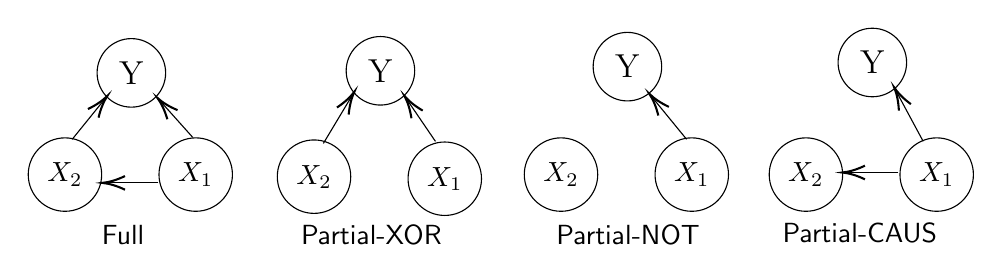
\begin{tikzpicture}[x=0.75pt,y=0.75pt,yscale=-1,xscale=1]
%uncomment if require: \path (0,270); %set diagram left start at 0, and has height of 270

%Straight Lines [id:da3925834327382034] 
\draw    (353,187) -- (366.97,163.71) ;
\draw [shift={(368,162)}, rotate = 120.96] [color={rgb, 255:red, 0; green, 0; blue, 0 }  ][line width=0.75]    (10.93,-3.29) .. controls (6.95,-1.4) and (3.31,-0.3) .. (0,0) .. controls (3.31,0.3) and (6.95,1.4) .. (10.93,3.29)   ;
%Straight Lines [id:da7616319252285488] 
\draw    (407,186) -- (393.13,165.65) ;
\draw [shift={(392,164)}, rotate = 55.71] [color={rgb, 255:red, 0; green, 0; blue, 0 }  ][line width=0.75]    (10.93,-3.29) .. controls (6.95,-1.4) and (3.31,-0.3) .. (0,0) .. controls (3.31,0.3) and (6.95,1.4) .. (10.93,3.29)   ;
%Straight Lines [id:da7468673133824906] 
\draw    (232,185) -- (247.74,165.55) ;
\draw [shift={(249,164)}, rotate = 128.99] [color={rgb, 255:red, 0; green, 0; blue, 0 }  ][line width=0.75]    (10.93,-3.29) .. controls (6.95,-1.4) and (3.31,-0.3) .. (0,0) .. controls (3.31,0.3) and (6.95,1.4) .. (10.93,3.29)   ;
%Straight Lines [id:da6450905490739657] 
\draw    (290,184) -- (274.33,166.49) ;
\draw [shift={(273,165)}, rotate = 48.18] [color={rgb, 255:red, 0; green, 0; blue, 0 }  ][line width=0.75]    (10.93,-3.29) .. controls (6.95,-1.4) and (3.31,-0.3) .. (0,0) .. controls (3.31,0.3) and (6.95,1.4) .. (10.93,3.29)   ;
%Straight Lines [id:da6658849542337637] 
\draw    (273.5,206) -- (248.5,206) ;
\draw [shift={(246.5,206)}, rotate = 360] [color={rgb, 255:red, 0; green, 0; blue, 0 }  ][line width=0.75]    (10.93,-3.29) .. controls (6.95,-1.4) and (3.31,-0.3) .. (0,0) .. controls (3.31,0.3) and (6.95,1.4) .. (10.93,3.29)   ;
%Straight Lines [id:da6301917918708001] 
\draw    (528,185) -- (511.27,164.55) ;
\draw [shift={(510,163)}, rotate = 50.71] [color={rgb, 255:red, 0; green, 0; blue, 0 }  ][line width=0.75]    (10.93,-3.29) .. controls (6.95,-1.4) and (3.31,-0.3) .. (0,0) .. controls (3.31,0.3) and (6.95,1.4) .. (10.93,3.29)   ;
%Straight Lines [id:da08700208498489559] 
\draw    (642,186) -- (628.95,161.76) ;
\draw [shift={(628,160)}, rotate = 61.7] [color={rgb, 255:red, 0; green, 0; blue, 0 }  ][line width=0.75]    (10.93,-3.29) .. controls (6.95,-1.4) and (3.31,-0.3) .. (0,0) .. controls (3.31,0.3) and (6.95,1.4) .. (10.93,3.29)   ;
%Straight Lines [id:da4870088229519337] 
\draw    (630,201) -- (605,201) ;
\draw [shift={(603,201)}, rotate = 360] [color={rgb, 255:red, 0; green, 0; blue, 0 }  ][line width=0.75]    (10.93,-3.29) .. controls (6.95,-1.4) and (3.31,-0.3) .. (0,0) .. controls (3.31,0.3) and (6.95,1.4) .. (10.93,3.29)   ;

% Text Node
\draw    (530.5, 202) circle [x radius= 17.69, y radius= 17.69]   ;
\draw (530.5,202) node    {$X_{1}$};
% Text Node
\draw    (467.5, 202) circle [x radius= 17.69, y radius= 17.69]   ;
\draw (467.5,202) node    {$X_{2}$};
% Text Node
\draw    (499.5, 150) circle [x radius= 16.51, y radius= 16.51]   ;
\draw (499.5,150) node  [font=\large]  {$\text{Y}$};
% Text Node
\draw    (411.5, 204) circle [x radius= 17.69, y radius= 17.69]   ;
\draw (411.5,204) node    {$X_{1}$};
% Text Node
\draw    (348.5, 203) circle [x radius= 17.69, y radius= 17.69]   ;
\draw (348.5,203) node    {$X_{2}$};
% Text Node
\draw    (380.5, 152) circle [x radius= 16.51, y radius= 16.51]   ;
\draw (380.5,152) node  [font=\large]  {$\text{Y}$};
% Text Node
\draw    (648.5, 202) circle [x radius= 17.69, y radius= 17.69]   ;
\draw (648.5,202) node    {$X_{1}$};
% Text Node
\draw    (585.5, 202) circle [x radius= 17.69, y radius= 17.69]   ;
\draw (585.5,202) node    {$X_{2}$};
% Text Node
\draw    (617.5, 148) circle [x radius= 16.51, y radius= 16.51]   ;
\draw (617.5,148) node  [font=\large]  {$\text{Y}$};
% Text Node
\draw    (291.5, 202) circle [x radius= 17.69, y radius= 17.69]   ;
\draw (291.5,202) node    {$X_{1}$};
% Text Node
\draw    (228.5, 202) circle [x radius= 17.69, y radius= 17.69]   ;
\draw (228.5,202) node    {$X_{2}$};
% Text Node
\draw    (260.5, 153) circle [x radius= 16.51, y radius= 16.51]   ;
\draw (260.5,153) node  [font=\large]  {$\text{Y}$};
% Text Node
\draw (245,225) node [anchor=north west][inner sep=0.75pt]   [align=left] {\textsf{Full}};
% Text Node
\draw (341,225) node [anchor=north west][inner sep=0.75pt]   [align=left] {\textsf{Partial-XOR}};
% Text Node
\draw (464,225) node [anchor=north west][inner sep=0.75pt]   [align=left] {\textsf{Partial-NOT}};
% Text Node
\draw (573,224) node [anchor=north west][inner sep=0.75pt]   [align=left] {\textsf{Partial-CAUS}};


\end{tikzpicture}
\caption{\label{fig:bn}Bayesian networks that we use as a schema to generate synthetic data, illustrating one full and three partial factorizations of $P(X,Y)$. %See examples in Table \ref{tab:types}.
        %\jcomment{@celia: update this}
}
\end{figure}
%\subsection{Feature Importance and Factors that Affect It}
We wish that the decision function of a model $f$ make predictions $\hat y = f(X)$ to minimize some expected loss; \[\mathbb{E}_{X,Y \sim P(Y,X)}[\ell(Y,f(X))]\] where $P(Y,X)$ is the data distribution and $\ell$ is some loss function. A decision function $f : \mathcal{X} \rightarrow \mathcal{Y}$ is essentially some function of $P(X,Y)$. For example, to maximize classification accuracy,
   \[
		y =  f(X) = %\argmaX_y P(y|x) = 
		 \argmax_y P(y|X)
   \]
Therefore, the feature importance outcome depends significantly on different mechanisms/properties of this generating distribution $P(X,Y)$. Namely, the properties of each variable (and its distribution), and the properties of the relations among variables. 
Considering only two features, we could represent the concept as a Bayesian network (Fig.~\ref{fig:bn} illustrates). 
%\jcomment{@celia: update this}
\[
	%P(X,Y) = P(X_1,X_2,Y) = P(X_2|X_1,Y)P(X_1|Y)P(Y)
    P(X,Y) = P(X_1,X_2,Y) = P(Y|X_1,X_2)P(X_2|X_1)P(X_1)
\]
i.e., a Full factorization of the joint, and thus we could consider the following properties (as nodes and edges): 
%\jcomment{@celia: update this}
\begin{enumerate}
	%\item $P(X_1)$: including type of feature (binary, categorical, continuous, %\ldots), and all aspects of its distribution (variance, imbalance, etc); 
	%\item $P(Y|X_1,X_2)$: specifying the amount and type of correlation between features and target, revealing the special case of $P(Y) = P(Y|X_1,X_2)$ when there is no correlation; and 
	%\item $P(X_1|X_2)$: amount of feature inter-dependence/co-correlation.
    \item $P(X_1)$: specifying the type of the feature $X_1$; 
    \item $P(X_2|X_1)$: the amount of conditional dependence of $X_2$ on $X_1$; and
	\item $P(Y|X_1,X_2)$: the amount and type of correlation between features and target, revealing the special case of $P(Y|X_1,X_2)=P(Y)$ when there is no correlation.
	
\end{enumerate}
%Different factorizations are of course possible, but this is the one we use to generate synthetic data. 
\textsf{Partial-XOR} and \textsf{Partial-NOT} exhibit feature independence (features are independent from each other -- when the target is observed), and both features are required to make a perfect prediction for \textsf{Partial-XOR}, and only $X_1$ is required to perfectly predict \textsf{Partial-NOT}; in this case deterministic.

In real-world settings,  \textsf{Full} represents the case where one feature is related to another feature and both participate to make the prediction of the output, for example in \textsc{Adult Income} dataset (that we later include in our experiments) the feature \textsc{occupation} is correlated to \textsc{age} and both predict the output \textsc{income}. \textsf{Partial-CAUS} on the other hand, may represent a causal relationship between one feature and the outcome through a chain of causality; or an indirect correlation of one feature on the output through another feature(or even multiple features), forming a chain of correlations.

\textsf{Full} and \textsf{Partial-CAUS} are specific cases of respectively \textsf{Partial-XOR} and \textsf{Partial-NOT} when $X_1$ is dependent on $X_2$, thus for the rest of this paper, we denote \textsf{XOR} to refer to both \textsf{Full} and \textsf{Partial-XOR}, and use \textsf{NOT} to refer to \textsf{Partial-CAUS} and \textsf{Partial-NOT}.
The data can be generated as:
%    \jcomment{@celia: update this}
%\begin{align}
    %y &\sim P(Y)\label{eq:y}\\
    %X_1 &\sim P(X_1) \label{eq:11} \\
    %X_2 &\sim P(X_2|X_1) \label{eq:21} \\
    %\epsilon &\sim P(\alpha_{\epsilon}|X_1,X_2) \label{eq:e1} \\
    %y &= f(X_1,X_2)
%\end{align}

\[
    P(X) \sim \mathcal{N}(\mu, \Sigma) 
\]

Where $\mathcal{N}$ is a bi-variate normal distribution and $\Sigma$ is the covariance matrix, representing the amount of correlation between the two random variables $X_1$ and $X_2$.
In order to introduce noise, we apply a mask to invert a percentage of labels in the output $y$. Let's denote the percentage of labels to invert as $\epsilon$. Let $M_i$ be a binary mask defined as:
\[ M_i = 
\begin{cases} \label{eq1}
1 & \text{with probability } \epsilon \\
0 & \text{with probability } 1-\epsilon
\end{cases}
\]
The perturbed output $y$ can be obtained with :
\[ \hat{y} = y \odot (1 - M) + (1 - y) \odot M \]
With $y=f(X)$ and $f$ represents the logical operators \textsf{XOR} or \textsf{NOT}.
%where $P(\alpha_{\epsilon}|X_1,X_2) \equiv \mathcal{B}(\alpha_{\epsilon})$, %when the target variable is continuous ($y \in \mathbb{R}$) and 
%$P(Y) \equiv \mathcal{B}(\alpha_y)$, and $P(X) \equiv \mathcal{N}(\mu, \Sigma)$, where $\Sigma$ is the covariance matrix. % and $P(X_2|X_1, Y) \equiv \mathcal{B}(\alpha_{X_2, X_1, y})$, 
%and $P(\epsilon | X_1,X_2) \equiv \mathcal{B}(\alpha_{X_1, X_2})$
%when $X_1$ and $X_2$ and the target $Y$ are binary ($X_1,X_2,Y \in \{0,1\}$). \\
%Varying $\epsilon$ control the amount of the irreducible noise and $\alpha_y$ controls the class imbalance in the generated data. 

%\jesse{Le reviewer dit "Another important limitation is the theoretical component. The paper is an empirical evaluation of 10 explainability methods. Instead, I suggest you understand the methods, and try to justify the final results obtained in the evaluations based on the advantages and disadvantages of each method. For example, why \textsf{LIME} and Global surrogates are not affected by the imbalance?". Il y a des tresors `cachés dans cette section. Parce que on imagine que `synthetic datasets' s'agit que de décrire des datasets. En fait, ce serait genial avoir une section `Theoretical Insights' ou `Discussion and Theoretical Insights'.}

\paragraph{Ground truth feature importance}\label{gtfi}
We use $\phi^*_{X}(f^*)$ to denote the ground truth feature importance that are given by the true model $f^*$ to which we compare $\phi_{X}(f)$, the feature importance estimates that is generated by each of the local explainability methods to explain the predictions of the learned model $f$.
Intuitively, the true model $f^*$ can be illustrated with a $D$-depth decision tree. With $D=2$ for \textsf{XOR} dataset variants (the first split on $X_1$ and the second on $X_2$) and $D=1$  for \textsf{NOT} dataset variants (only one split on $X_1$).

When $\epsilon = 0$, the ground truth feature importance $\phi^{\star}_{X}$ for all variants of \textsf{XOR} datasets are fixed as $\phi^{\star}_{X_1}$ = $\phi^{\star}_{X_2}$ = .5, because both $X_1$ and $X_2$ are \emph{necessary} to make the prediction of \textsf{XOR}. The amount of the correlation $\rho$ between $X_1$ and $X_2$ doesn't affect the importance as both are \emph{necessary} to make the prediction of \textsf{XOR}. Meanwhile, only $X_1$ is \emph{necessary} to make the prediction of \textsf{NOT}, thus $\phi^{\star}_{X_1}$ = 1 and $\phi^{\star}_{X_2}$ = $\rho$, because when $X_2$ is correlated to $X_1$, $X_2$ have an indirect influence estimated by $\rho$ to predict \textsf{NOT}. 

On the other hand, when $\epsilon \neq 0$, $\phi^{\star}_{X_1} = \phi^{\star}_{X_2} = .5 * \epsilon$ for \textsf{XOR} dataset variants, and $\phi^{\star}_{X_1} = 1 * \epsilon$ and $\phi^{\star}_{X_2} = \rho * \epsilon$ for \textsf{NOT} dataset variants.

%The amount of the correlation $\rho$ between $X_1$ and $X_2$ doesn't affect the importance as both are necessary to make the prediction of \textsf{XOR}. For \textsf{NOT}, only $X_1$ is necessary for the prediction, thus $\phi^{\star}_{X_2}=0$ for $\rho=0$ and $\phi^{\star}_{X_2}=\rho$ otherwise.

%To measure the similarity between two vectors (e.g., between two sets of explanations or between an explanation and the true model weights), we use L1 distance and cosine distance. L1 distance ranges between [0, ) and is 0 when two vectors are the same. Cosine distance ranges between [0, 2] and is 0 when the angle between two vectors is 0 (or 360). For both metrics, the lower the value, the more similar two given vectors are.

%$1 & \text{if} x_1 \neq x_2$ 
%$0 & \text{if } x_1 = x_2$
%\end{cases} \]
For the XOR function, both \(x_1\) and \(x_2\) are equally important in determining the output, and their importance scores should ideally converge to \(0.5\) when considering a large amount of data points.
Consider a decision tree model that aims to predict the XOR function using features \(x_1\) and \(x_2\). For simplicity, let's assume that the decision tree splits on both \(x_1\) and \(x_2\) at each level. The decision tree's predictions can be expressed as:
\[ \hat{y} = f(x_1, x_2) \]
Now, let's define the feature importance scores (\(\phi_{x_1}\) and \(\phi_{x_2}\)) using the Gini impurity criterion, a common metric for decision trees:
\[ \phi_{x_1} = \sum_{\text{nodes splitting on } x_1} \text{Gini decrease at the node} \]
\[ \phi_{x_2} = \sum_{\text{nodes splitting on } x_2} \text{Gini decrease at the node} \]
In a large dataset, the decision tree will be able to accurately capture the XOR relationship, and both \(x_1\) and \(x_2\) should contribute equally to the impurity decrease, leading to similar importance scores. For a balanced decision tree, these Gini decreases would be distributed among the splits involving \(x_1\) and \(x_2\). In the limit of a large dataset, we would expect:
\[ \lim_{{\text{large dataset}}} \phi_{x_1} = \lim_{{\text{large dataset}}} \phi_{x_2} = 0.5 \]
This indicates that, as the dataset size increases, the decision tree's feature importance for predicting the XOR function would converge to \(0.5\) for both \(x_1\) and \(x_2\), reflecting their equal importance in determining the output.

\section{Empirical Setup}
To carry out our experiments, we demonstrate our findings on four real-world datasets: \textsc{Heart Diagnosis}, \textsc{Cervical Cancer}, \textsc{Adult Income} and \textsc{German Credit Risk}. These datasets include properties such as feature interactions (dependence or independence),% mixtures of feature types (such as binary and continuous), feature distributions (such as Bernoulli and Gaussian), 
noise, random irrelevant variables and class imbalance. %Figure \ref{propertiesheart} illustrates an example of feature distributions on the Heart dataset.
%\begin{figure}[h] \label{propertiesheart}
%  \centering
  %\includegraphics[width=350pt, height=250pt]{fig/heart.png}
  %\includegraphics[width=500pt, height=180pt]{figs/cancerfiwr.png}
   %\includegraphics[width=500pt, height=180pt]{figs/cancerficorr.png}
%  \caption{Illustration of feature distributions for Heart dataset.%\jcomment{Nice. For the feature interactions that include one discrete variable and one continuous variable, I wonder if a box plot or `violin plot' might help the visualization -- but that is an optional extra; these plots already tell a nice story.}
%  }
%\end{figure}

We generate 24 synthetic datasets (Figures \ref{synthdata} and \ref{synthdata2}) expressing different combinations of these properties by varying several parameters such as the correlation amount of the normal distribution from which the data points are drawn and the probability of each class, thus, the amount of generated noise and class imbalance. %We also use $X_3$ as an irrelevant variable in order to quantify how feature importance scorers are sensitive to random irrelevant variables.
Each dataset is divided to 80\% for training and 20\% for testing. We report the results of the feature importance estimates on the test set. 
We compute feature importance estimates on the true model $f^*$ and learned model $f$, so that we can compare the generated feature importance estimates to their ground truth values.
Finally, we analyze the advantages and limitations of each explainability method on the synthetic datasets and we run larger experiments on the above real-world datasets from the UCI repository \cite{Dua:2019}. 
%\jcomment{2nd main suggestion: For the real-world datasets, why not vary the amount of data from 10\%, 20\% ,... 100\%. Also, identify/estimate/quantify for every single feature the type of feature it represents (dependence wrt target variable and wrt other features). Generally (possibly non-linear) dependence is difficult to estimate, but an estimate would suffice.}
%\jesse{Un reviewer: "How to evaluate the model's prediction accuracies? Cross validation or holdout estimate? Anyway, these important details were missing apparently." Normalmente un trouve cette information ici.}

\begin{figure*}
  %\vspace*{-1in}
  %\hspace*{-1in}
  \centering
  %\includegraphics[width=1.3\textwidth]{figures/contdt1000.png}
  \includegraphics[width=1.1\textwidth]{figures/xorcontdt1000.png}
  %\includegraphics[width=\textwidth]{figures/datanot.png}
  %\vspace*{-2.5cm}
  \caption{\label{synthdata} Synthetic data XOR. $X \sim \mathcal{N}(\mu, \Sigma)$. Each dataset expresses a different combination of properties. }
\end{figure*}
\begin{figure*}
  %\vspace*{-1in}
  %\hspace*{-1in}
  \centering
  %\includegraphics[width=1.3\textwidth]{figures/contdt1000.png}
  %\includegraphics[width=\textwidth]{figures/dataxor.png}
  \includegraphics[width=1.1\textwidth]{figures/notcontdt1000.png}
  %\vspace*{-2.5cm}
  \caption{\label{synthdata2} Synthetic data NOT. $X \sim \mathcal{N}(\mu, \Sigma)$. Each dataset expresses a different combination of properties. }
\end{figure*}

\subsection{Datasets, models and metrics}
\paragraph{Datasets}
%\textsf{XOR} and \textsf{NOT} correspond to the logical operations of the same names performed on $X_1$ and $X_2$ in the case of \textsf{XOR} and on $X_1$ in the case of \textsf{NOT}. \textsf{XOR} and \textsf{NOT} can be respectively represented with the \textsf{Full} and \textsf{Partial-CAUS} networks when $X_1$ and $X_2$ are correlated and by the \textsf{Partial-XOR} and \textsf{Partial-NOT} networks otherwise.
Figures \ref{synthdata} and \ref{synthdata2} show the generated datasets by varying the parameters in Eq~\ref{eq1}: 
$\mu \in \{[0,1],[1,0]\}$, $\Sigma \in \{ [[1, 0], [0, 1]], [[1, .1], [.1, 1]] , [[1, .9], [.9, 1]], [[1, 1], [1, 1]] \}$, and $\epsilon \in \{0, .25, .5\}$.

%While Caus- expresses the properties of Chain, XOR and NOT are two examples of respectively Hub and Spoke networks in Figure \ref{fig:bn}.
%\jesse{Un reviewer evoque "There is also a question about the evaluation approach used in this study. The evaluation is conducted in the following steps: (i) generating data, (ii) tarining Random Forest with the generated data, (iii) applying the feature attribution methods to the trained Random Forest, and (iv) comparing the data generation process and the results of the feature attribution methods. One problem with this approach is that the "quality of the trained Random Forest" and the "quality of the feature attribution method" are mixed together. The authors used the inconsistency between the data generating process and the results of feature attribution for performance evaluation. However, \textbf{if the trained Random Forest does NOT reflect the data generating process properly, even if the results of feature attribution are inconsistent with the process, it is not necessarily a problem with the feature attribution method}. For at least the eight model-agnostic methods, \textbf{it would be more appropriate to use the data generating process directly as a model and apply the feature attribution methods to it}. This will enable a more appropriate performance evaluation without the uncertainty introduced by the training of Random Forest. For Random Forest-specific evaluation (although the motivation is not clear), it is necessary to appropriately distinguish between the "quality of the trained Random Forest'' and the "quality of the feature attribution method", and to develop a method to evaluate only the latter." [my emphasis, JR]. Comme j'ai évoqué une autre fois : l'atout de générer nos propres données est qu'on connaît la 'ground truth'. C'est pour ça que je suggère 1) montrer quelques datasets synthétiques (par exemple, dans des figures); 2) déclarer ce qu'est la ground truth (the *true* feature importance estimates *of the data*); et peut-être 3) démontrer les prédictions de RF sur ces données. }
%Table~\ref{tab:types} summarizes some examples that we consider later in the experiments. 
%On the other hand, Caus expresses another factorization where $X_1$ is dependent on $y$ and $X_2$. Such a case could occur in the real-world where there is a Causal relationship between two features. For example when modeling if a sprinkler should be triggered or not based on whether the grass is wet or not which is dependent on rain. 
%Figure \ref{Caus} illustrates this Causal relationship.
%\begin{table}[tb]
%\begin{small}
%\begin{tiny}
%	\centering
%    \resizebox{\columnwidth}{!}{
%	\begin{tabular}{|l|c|c|c|}
%		\hline
%		$f(X_1,X_2)$  & $P(X_1|Y)$ & $P(X2|X_1,Y)$ & Independence \\
%		\hline
%		 XORdisc & $\mathcal{B}(\alpha_{X_1,y})$ & $\mathcal{B}(\alpha_{X_2,y})$ & $X_1\indep X_2 \mid Y$,$Y\dep X_1,X_2$ \\
%		 XORcont & $\mathcal{N}(\mu_{X_1, y}, \sigma_{X_1, y})$ & $\mathcal{N}(\mu_{X_2, y}, \sigma_{X_2, y})$ & $X_1\indep X_2\mid Y$ , $Y\dep X_1,X_2$ \\
%		 Not($X_1$)-disc & $\mathcal{B}(\alpha_{X_1,y})$ & $\mathcal{B}(\alpha_{X_2})$ & $X_1 \indep X_2 \mid Y$, $Y \dep X_1$, $Y \indep X_2$  \\
%         Not($X_1$)-cont & $\mathcal{N}(\mu_{X_1, y}, \sigma_{X_1, y})$ & $\mathcal{N}(\mu_{X_2}, \sigma_{X_2})$ &  $X_1 \indep X_2 \mid Y$, $Y \dep X_1$, $Y \indep X_2$   \\
         %Full-disc & $\mathcal{B}(\alpha_{X_1,y})$ & $\mathcal{B}(\alpha_{X_2,X_1,y})$ & $X_2 \dep X_1 \mid Y$, $Y \dep X_1, X_2$  \\
         %Full-cat & $\mathcal{M}(k,\alpha_{X_1,y})$ & $\mathcal{M}(k,\alpha_{X_2,X_1,y})$ &  $X_2 \dep X_1 \mid Y$, $Y \dep X_1, X_2$ \\
         %Full-cont & $\mathcal{N}(\mu_{X_1, y}, \sigma_{X_1, y})$  & $\mathcal{N}(\mu_{X_2,X_1, y}, \sigma_{X_2,X_1, y})$  &  $X_2 \dep X_1 \mid Y$, $Y \dep X_1, X_2$ \\
         %Full-mix & $\mathcal{B}(\alpha_{X_1,y})$ & $\mathcal{N}(\mu_{X_2, y}, \sigma_{X_2, y})$ & $X_2 \dep X_1 \mid Y$, $Y \dep X_1, X_2$ \\
         %Full-mixGaus & $\mathcal{N}(\mu_{X_1, y}, \sigma_{X_1, y})$ & $\mathcal{N}(\mu_{X_2,X_1, y}, \sigma_{X_2,X_1, y})$ & $X_2 \dep X_1 \mid Y$, $Y \dep X_1, X_2$ \\
         %Caus-disc & $\mathcal{B}(\alpha_{X_1,y})$ & $\mathcal{B}(\alpha_{X_2, X_1})$ & $X_1 \dep X_2 \mid Y$, $Y \dep X_1$, $Y \indep X_2$  \\
         %Caus-cont & $\mathcal{N}(\mu_{X_1, y}, \sigma_{X_1,y})$ & $\mathcal{N}(\mu_{X_2, X_1}, \sigma_{X_2, X_1})$ & $X_1 \dep X_2 \mid Y$, $Y \dep X_1$, $Y \indep X_2$ \\
         %Gaus-cat & $\mathcal{M}(k,\alpha_{X_1,y})$ & $\mathcal{M}(k,\alpha_{X_2, X_1})$ & $X_1 \dep X_2 \mid Y$, $Y \dep X_1$, $Y \indep X_2$ \\
         %Caus-mix & $\mathcal{B}(\alpha_{X_1,y})$ & $\mathcal{N}(\mu_{X_2, X_1}, \sigma_{X_2, X_1})$ & $X_1 \dep X_2 \mid Y$, $Y \dep X_1$, $Y \indep X_2$ \\
%		\hline
%	\end{tabular}
% }
%\end{tiny}
%\end{small}
 %\caption{\label{tab:types}Examples of different properties/mechanisms that we consider for generating synthetic data; $\mathcal{B}$ is the Bernoulli distribution, $\mathcal{M}$ is the Multinoulli distribution and $\mathcal{N}$ is the normal distribution. $Y$ is drawn from a $\mathcal{B}$ and $X_3$ is an irrelevant feature, drawn independently either from a $\mathcal{B}$ or $\mathcal{N}$. Varying $\alpha$ of $\mathcal{B}$, $\alpha$ and $k$ of $\mathcal{M}$ and the $\mu$ and $\sigma$ of $\mathcal{N}$ (also the mixture of Gaussians) controls the amount of class imbalance and the noise generated. The generation of each feature is conditioned on the value of $Y$, for example $X_1$ is drawn from $\mathcal{B}(\alpha_{X_1}^0)$ for $y==0$ and $\mathcal{B}(\alpha_{X_1}^1)$ for $y==1$. %kajouter k (k=[5, 10, 100], ajouet 100 instance, changer alpha en p pour distinguer 
 %   }
%\end{table}

%Thus, the quality of the feature importance generated sh
%\jesse{Un reviewer: "The paper's model only handles two variables. I understand that this simplicity matters to systematically understand the model behaviors, but this would also devalue/limit the practical value of the paper's outcomes because we need to handle high-dimensional data in many situations. This is caused by considering many factors (i.e. many variables) at a time, and we tend to feed many input variables to an ML analysis. As a result, we need to consider the correlation (or collinearity) among input variables because it is quite difficult to prepare many but no-correlating variables. Nevertheless, any 'feature attribution' tries to project multi-dimensional correlations into each single-variable contribution and thus every method for it should be lossy (every method needs to have information loss).". On a parlé déjà une fois sur l'idée d'avoir un jeu de données avec plusieurs variables ... peut-être on peut reprendre cette discussion la prochaine réunion. }

In addition, Table \ref{tab:datasets} summarizes the properties of the four real-world datasets that we use to demonstrate our findings.
\begin{table}[h]
%\begin{tiny}
	\centering
    \resizebox{\columnwidth}{!}{
	\begin{tabular}{|l|c|c|c|c|c|}
		\hline
		Dataset & $\#$instances & $\#$features & $\%$ discrete & $\%$ continuous & imbalance \\
		\hline
		  \textsc{Heart Diagnosis} & 303 & 13 & 43 & 57 & yes \\
          \textsc{Cervical Cancer} & 858 & 35 & 62 & 38 & yes \\
          %Compas & 7214 & 52 & discrete, continuous  & yes \\
          \textsc{Adult Income}& 32561 & 11 & 65 & 35 & no\\
          \textsc{German Credit Risk} & 1\,000 & 23 & 70 & 30 & yes \\ 
		\hline
	\end{tabular}
 }
 \caption{\label{tab:datasets} Summary of the real-world datasets we include in our experiments.}
% \end{tiny}
\end{table}
%\textcolor{red}{maybe add correlation matrices  and say if there are irrelevant variables and irreducible noise ??}
\paragraph{Models}
%For each dataset, we train four models: a simple model (linear regression for the WHO dataset and logistic regression for the HELOC dataset) that can satisfy conditions of the guiding principle and three more complex models (neural networks of varying complexity) that are more reflective of real-world applications. Model architectures and performance are described in Appendix A.5.
For the synthetic datasets, we compute the feature importance scores of %two models: the true model $f^*$ that can be expressed as a decision tree with maximum depth set to 2 and trained on datasets with 50\,000 instances for each, and 
the learned model $f$ on datasets with 1\,000 instances. The learned model $f$ can be either a decision tree or a random forest.%with 10 estimators, each with 2-depth a
%\textit{maxdepth=2, nestimators=10, randomstate=0, maxfeatures='sqrt'}
%The feature importance estimates of the decision tree converges to the ground truth feature importance when the number of generated instances = 50\,000. We report the results on the decision tree in the main paper and those achieved using the random forest can be found in Table \ref{datasetss50K} in Appendix \ref{secb}. 
On the other hand, we use the random forest model with parameters learned using grid search and evaluated with 10-fold cross-validation for each of the real-world datasets. Table \ref{datasetss} summarizes the performances and the feature importance of the decision tree and the random forest models for the generated datasets.
\begin{table}[h]
    \centering
    \resizebox{\columnwidth}{!}{
    \begin{tabular}{|l|c|c|c|c|c|c|}
\hline
Decision function &  $\epsilon$ &  $\rho$ &  DT Accuracy &     DT feature importance &  RF Accuracy &     RF feature importance \\
\hline
              \textsf{XOR} &        0.00 &    0.00 &         1.00 & $\phi_{X_1}$=0.44, $\phi_{X_2}$=0.56 &         0.85 & $\phi_{X_1}$=0.69, $\phi_{X_2}$=0.31 \\
              \textsf{XOR} &        0.00 &    0.10 &         1.00 & $\phi_{X_1}$=0.41, $\phi_{X_2}$=0.59 &         0.90 & $\phi_{X_1}$=0.63, $\phi_{X_2}$=0.37 \\
              \textsf{XOR} &        0.00 &    0.90 &         1.00 & $\phi_{X_1}$=0.51, $\phi_{X_2}$=0.49 &         1.00 & $\phi_{X_1}$=0.55, $\phi_{X_2}$=0.45 \\
              \textsf{XOR} &        0.00 &    1.00 &         1.00 &   $\phi_{X_1}$=0.5, $\phi_{X_2}$=0.5 &         1.00 & $\phi_{X_1}$=0.53, $\phi_{X_2}$=0.47 \\
              \textsf{XOR} &        0.25 &    0.00 &         0.70 & $\phi_{X_1}$=0.47, $\phi_{X_2}$=0.53 &         0.61 & $\phi_{X_1}$=0.62, $\phi_{X_2}$=0.38 \\
              \textsf{XOR} &        0.25 &    0.10 &         0.72 &   $\phi_{X_1}$=0.4, $\phi_{X_2}$=0.6 &         0.62 & $\phi_{X_1}$=0.64, $\phi_{X_2}$=0.36 \\
              \textsf{XOR} &        0.25 &    0.90 &         0.72 & $\phi_{X_1}$=0.51, $\phi_{X_2}$=0.49 &         0.72 & $\phi_{X_1}$=0.56, $\phi_{X_2}$=0.44 \\
              \textsf{XOR} &        0.25 &    1.00 &         0.71 & $\phi_{X_1}$=0.51, $\phi_{X_2}$=0.49 &         0.71 & $\phi_{X_1}$=0.53, $\phi_{X_2}$=0.47 \\
              \textsf{XOR} &        0.50 &    0.00 &         0.52 & $\phi_{X_1}$=0.83, $\phi_{X_2}$=0.17 &         0.50 & $\phi_{X_1}$=0.57, $\phi_{X_2}$=0.43 \\
              \textsf{XOR} &        0.50 &    0.10 &         0.53 & $\phi_{X_1}$=0.69, $\phi_{X_2}$=0.31 &         0.56 & $\phi_{X_1}$=0.57, $\phi_{X_2}$=0.43 \\
              \textsf{XOR} &        0.50 &    0.90 &         0.49 & $\phi_{X_1}$=0.64, $\phi_{X_2}$=0.36 &         0.46 & $\phi_{X_1}$=0.53, $\phi_{X_2}$=0.47 \\
              \textsf{XOR} &        0.50 &    1.00 &         0.54 & $\phi_{X_1}$=0.55, $\phi_{X_2}$=0.45 &         0.47 & $\phi_{X_1}$=0.53, $\phi_{X_2}$=0.47 \\
\hline  
              \textsf{NOT} &        0.00 &    0.00 &         1.00 &   $\phi_{X_1}$=1.0, $\phi_{X_2}$=0.0 &         1.00 & $\phi_{X_1}$=0.84, $\phi_{X_2}$=0.16 \\
              \textsf{NOT} &        0.00 &    0.10 &         1.00 &   $\phi_{X_1}$=1.0, $\phi_{X_2}$=0.0 &         1.00 & $\phi_{X_1}$=0.83, $\phi_{X_2}$=0.17 \\
              \textsf{NOT} &        0.00 &    0.90 &         1.00 &   $\phi_{X_1}$=1.0, $\phi_{X_2}$=0.0 &         1.00 & $\phi_{X_1}$=0.61, $\phi_{X_2}$=0.39 \\
              \textsf{NOT} &        0.00 &    1.00 &         1.00 &   $\phi_{X_1}$=1.0, $\phi_{X_2}$=0.0 &         1.00 & $\phi_{X_1}$=0.49, $\phi_{X_2}$=0.51 \\
              \textsf{NOT} &        0.25 &    0.00 &         0.72 &   $\phi_{X_1}$=1.0, $\phi_{X_2}$=0.0 &         0.72 & $\phi_{X_1}$=0.77, $\phi_{X_2}$=0.23 \\
              \textsf{NOT} &        0.25 &    0.10 &         0.69 & $\phi_{X_1}$=0.99, $\phi_{X_2}$=0.01 &         0.72 &   $\phi_{X_1}$=0.8, $\phi_{X_2}$=0.2 \\
              \textsf{NOT} &        0.25 &    0.90 &         0.71 &   $\phi_{X_1}$=1.0, $\phi_{X_2}$=0.0 &         0.71 & $\phi_{X_1}$=0.63, $\phi_{X_2}$=0.37 \\
              \textsf{NOT} &        0.25 &    1.00 &         0.72 & $\phi_{X_1}$=0.97, $\phi_{X_2}$=0.03 &         0.72 & $\phi_{X_1}$=0.49, $\phi_{X_2}$=0.51 \\
              \textsf{NOT} &        0.50 &    0.00 &         0.50 & $\phi_{X_1}$=0.39, $\phi_{X_2}$=0.61 &         0.48 & $\phi_{X_1}$=0.55, $\phi_{X_2}$=0.45 \\
              \textsf{NOT} &        0.50 &    0.10 &         0.58 &   $\phi_{X_1}$=0.0, $\phi_{X_2}$=1.0 &         0.57 &   $\phi_{X_1}$=0.5, $\phi_{X_2}$=0.5 \\
              \textsf{NOT} &        0.50 &    0.90 &         0.50 & $\phi_{X_1}$=0.69, $\phi_{X_2}$=0.31 &         0.46 & $\phi_{X_1}$=0.53, $\phi_{X_2}$=0.47 \\
              \textsf{NOT} &        0.50 &    1.00 &         0.48 & $\phi_{X_1}$=0.49, $\phi_{X_2}$=0.51 &         0.50 & $\phi_{X_1}$=0.51, $\phi_{X_2}$=0.49 \\
\hline
\end{tabular}
}
    \caption{Parameterization and performances of the decision tree (DT) and the random forest (RF) for the 24 generated datasets with 1.000 instances. Maximum depth of both DT and RF is set to 2.
    % The decision tree corresponds to our generative model of the datasets. 
     %DT and RF parameters: maxdepth=2, nestimators=10, randomstate=0, maxfeatures='sqrt'.
     %DT and RF learning are extremely affected by the noise.
     }
    \label{datasetss}
\end{table}
\paragraph{Metrics}
To evaluate the quality of the feature importance estimates attributed by the methods in Table \ref{tab:accr}, we compare the feature importance estimates to the ground truth feature importance in Section \ref{gtfi} of the synthetic datasets because the ground truth feature importance estimates in the real-world datasets are hard to obtain. We also evaluate the stability, compactness, consistency, feature and rank agreements for the synthetic and real-world datasets.




\subsection{Experiments}
\subsubsection{Synthetic data}
%Since we have access to the ground truth feature importance for the synthetic datasets, we first compare the feature importance estimates given by the six methods in Table \ref{tab:accr} to the ground truth values provided in Section \ref{gtfi}. 
Figures \ref{boxplotxor} and \ref{boxplotnot} show the normalized feature importance estimates attributed by the selected explainability methods. After the normalization of the absolute importance of $X_1$ and $X_2$, their contributions sum to one. We perform the normalization to faithfully compare the feature attributions to their ground truth values. 

\paragraph{Explainability methods based on learning surrogate models overestimate the importance to irrelevant variables, Tree interpreter is sensitive to noise and SHAP explainers always favor one feature over the other} 
Overall, all explainers except local surrogates overestimate the importance of $X_1$ over $X_2$ across the \textsf{XOR} datasets. Also, none of these methods perfectly matches ground truth feature importance on average across all datasets.
Moreover, \textsf{LSurro} and \textsf{LIME} feature importance attributions are the least affected by noise and feature correlation. Indeed, \textsf{LSurro} and and \textsf{LIME} attribute comparable importance to $X_1$ and $X_2$ for \textsf{XOR} and \textsf{NOT} dataset variants, and both overestimate the importance of unimportant features (such as $X_2$ in case of \textsf{NOT}). 
Notably, \textsf{TI} is the most affected by noise, that is confirmed in its decomposition of the the feature and noise contributions to the prediction.
Additionally, feature correlations increase the importance and instability of $X_2$ importance in \textsf{XOR} datasets attributed by \textsf{SHAP} explainers, and noise lowers the importance of $X_1$ and $X_2$ for all the explainers.
Finally, \textsf{SHAP} explainers and \textsf{TI} have the highest variance of feature importance estimates in the \textsf{NOT} datasets.


%\begin{figure*}
%  %\centering
%  \includegraphics[width=\textwidth]{figures/boxplot.png}
%  \caption{\label{boxplot} Normalized feature importance with min-max standardization on the 24 generated datasets. These feature importance are obtained for the decision trees trained on datasets with 1\,000 instances.}
%\end{figure*}

\begin{figure*}
  %\vspace*{-1in}
  %\hspace*{-1in}
  \centering
  \includegraphics[width=1.1\textwidth]{figures/xorboxplot.png}
  %\vspace*{-1cm}
  \caption{\label{boxplotxor} Normalized feature importance estimates of the \textsf{XOR} datasets. These feature importance estimates are obtained for the decision trees trained on datasets with 1\,000 instances.}
\end{figure*}

\begin{figure*}
  %\vspace*{-1in}
  %\hspace*{-1in}
  \centering
  \includegraphics[width=1.1\textwidth]{figures/notboxplot.png}
  %\vspace*{-1cm}
  \caption{\label{boxplotnot} Normalized feature importance estimates of the \textsf{NOT} datasets. These feature importance estimates are obtained for the decision trees trained on datasets with 1\,000 instances. }
\end{figure*}
%compare to dt coefs ?????????
%\paragraph{Robustness against class imbalance, noise and irrelevant variables}    
%For each dataset, we train four models: a simple model (linear regression for the WHO dataset and logistic regression for the HELOC dataset) that can satisfy conditions of the guiding principle and three more complex models (neural networks of varying complexity) that are more reflective of real-world applications. Model architectures and performance are described in Appendix A.5.


\paragraph{SHAP explainers yield very comparable explanations}
Figure \ref{frag} shows the faithfulness of the explanations to the ground truth measured by mean consistency and mean feature agreements across the \textsf{XOR} and \textsf{NOT} generated datasets.
%For each dataset, we train four models: a simple model (linear regression for the WHO dataset and logistic regression for the HELOC dataset) that can satisfy conditions of the guiding principle and three more complex models (neural networks of varying complexity) that are more reflective of real-world applications. Model architectures and performance are described in Appendix A.5.


\begin{figure}[h]
  \vspace*{-.5in}
  %\hspace*{-1in}
  \centering
  %\includegraphics[width=\textwidth/4]{figures/featagremxor.png}
  %\includegraphics[width=\textwidth/4]{figures/featagremnot.png}
   \includegraphics[width=\textwidth/3]{figures/rankagremxor.png}
   \includegraphics[width=\textwidth/3]{figures/rankagremnot.png}
   \includegraphics[width=\textwidth/3]{figures/consistencyxor.png}
  \includegraphics[width=\textwidth/3]{figures/consistencynot.png}

  \caption{\label{frag}Mean consistency, mean feature agreements for \textsf{XOR} and \textsf{NOT} datasets. Consistency is expressed in $L_2$ distance (the lower the better). Feature agreement measures the fraction of common features between the sets of top-k features of the two rankings (the higher the better). %Rank agreement checks that the feature order is comparable between the two rankings (the higher the better). 
  }
\end{figure}


\textsf{SHAP} explainers yield consistent explanations due to the same feature importance attribution mechanism they all employ. However their explanations are the most inconsistent with respect to the ground truth values. 
Furthermore and for both \textsf{XOR} and \textsf{NOT} datasets, on average the fraction of common feature importance between \textsf{TI} and \textsf{KShap} and between \textsf{SShap} and \textsf{TShap} match perfectly. 

%\item Rank agreement:  \textsf{SHAP} explainers have perfect feature ranking across all datasets. While \textsf{TI} is the least similar to the ground truth for the \textsf{XOR} datasets and \textsf{TI} and \textsf{Tshap} are the least comparable to ground truth feature importance values. 


\begin{table}[h]
    \centering
    \resizebox{\columnwidth}{!}{
     \begin{tabular}{|l|c|c|c|c|c|}
    \hline
    function &  Methods  & \# Features for 90\% approximation & Distance with 1 feature(\%) & Mean consistency & Mean Stability (10) \\
    \hline  
    \textsf{XOR} & \textsf{Kshap} &       1.00       &       0.10       &  0.21    &  0.21  \\
    \textsf{XOR} & \textsf{Sshap} &       1.00      &        0.11       &  0.23    &  0.24   \\
    \textsf{XOR} & \textsf{Tshap} &       1.00      &        0.10       &  0.24    &  0.25  \\
    \textsf{XOR} & \textsf{TI} &          1.00      &        0.17       &  0.26    &  0.24   \\
    \textsf{XOR} & \textsf{LIME} &        1.00    &          0.16       &  0.28    &  0.33   \\
    \textsf{XOR} & \textsf{LSurro} &      1.33     &         0.43       &  0.32    &  0.15   \\   
     \hline
    \textsf{NOT} & \textsf{Kshap} &        1.00     &         0.03           &  0.14    &  0.16  \\
    \textsf{NOT}& \textsf{Sshap} &         1.00         &     0.03           &  0.15    &  0.20   \\
    \textsf{NOT}& \textsf{Tshap} &         1.00      &        0.03           &  0.19    &  0.19   \\
    \textsf{NOT}& \textsf{TI} &            1.00    &          0.02           &  0.15    &  0.19   \\
    \textsf{NOT}& \textsf{LIME} &          1.00       &       0.04           &  0.17    &  0.27   \\
    \textsf{NOT}& \textsf{LSurro} &        1.17      &        0.30        &  0.25    &   0.08  \\ 
    \hline
    \end{tabular}}
    \caption{Compactness and stability of the explanations for the \textsf{XOR} datasets. \textsf{Tshap} and \textsf{TI} are the most stable explainers for \textsf{XOR} and \textsf{LSurro} uses only one feature to make nearly half of the prediction of \textsf{NOT}.}
    \label{perfsxor}
\end{table}

% \begin{table}[h]
%    \centering
%    \resizebox{\columnwidth}{!}{
%     \begin{tabular}{|l|c|c|c|c|}
 %   \hline
 %   Methods  & \# Features for 90\% approximation & Distance with 1 feature(\%) & Mean consistency & Mean Stability \\
   
%    \hline
%    \end{tabular}}
%    \caption{Compactness and stability of the explanations for the \textsf{NOT} datasets. %Compactness measures how close we want to be to the reference model with all features? and how many features are selected to evaluate the approximation ?. Stability : the average variability of the feature across the instances' neighborhood.
%    }
%    \label{perfsnot}
%\end{table}
\paragraph{\textsf{LSurro} is the most locally stable, overestimates unimportant features and achieves better model accuracy with less features}
Table \ref{perfsxor} shows mean consistency, mean stability and compactness across the \textsf{XOR} and \textsf{NOT} datasets.
For \textsf{XOR} and \textsf{NOT} datasets respectively, \textsf{Kshap} is the most consistent to the rest of the explanatory methods on average.
Additionally, on average, \textsf{LSurro} generates the most locally stable explanations in \textsf{XOR} and \textsf{NOT} datasets, achieves higher model estimation and often consider both features as important fr both datasets.


\subsubsection{Real-world data}
For the real-world datasets the ground truth feature importance is unavailable, we perform evaluation of the different metrics in Section \ref{metrics}.

\paragraph{Local surrogates achieves 100\% of model accuracy with 5 features on \textsc{Adult Income} dataset.}
Figure \ref{adult} shows feature agreements for \textsc{Adult Income} Income dataset. 
\textsf{Kshap} and \textsf{Sshap} have exactly the same top-10 feature attributions and ranking. \textsf{TI} and \textsf{Tshap} share the same set of top-10 features. The rest of the explainers share 90\% of the top 10 most important features.
\textsf{LIME} share the lowest of top-10 important features with TI, \textsf{Kshap} and \textsf{Sshap} on the ranking of the top 10 features.
Additionally, Table \ref{adult2} illustrates the compactness, mean consistency and stability of the different methods on the \textsc{Adult Income} Income dataset. \textsf{LSurro} explains 100\% of model output with only 5 features. \textsf{Kshap}, \textsf{Tshap} and \textsf{TI} are the most stable for this dataset and \textsf{LIME} have the highest mean consistency across all the datasets.
\begin{figure}[h]%
  \centering
  \includegraphics[width=\textwidth/3]{figures/featagremAdult1.png}
  \includegraphics[width=\textwidth/3]{figures/rankagremAdult1.png}
  \caption{Feature and rank agreements for \textsc{Adult Income} Income dataset. }\label{adult}
\end{figure}

\begin{table}[h]
    \centering
    \resizebox{\columnwidth}{!}{ 
    \begin{tabular}{|l|c|c|c|c|}
    \hline
    Methods  & \# Features for 90\% Accuracy & Accuracy with 5 feature(\%) & Mean consistency & Mean Stability \\
    \hline
    \textsf{Kshap} &          \textbf{1} &          09 &  0.43 & \textbf{0.00}\\
    \textsf{Tshap} &         \textbf{1} &          09 & 0.43  & \textbf{0.00} \\
    \textsf{Sshap} &        \textbf{1}&          08 &  0.43 & 0.01 \\
    \textsf{LIME} &         \textbf{1} &          07 & \textbf{0.15}  & 0.07 \\
    \textsf{TI} &          \textbf{1}&          10 &  0.5    &  \textbf{0.00} \\
    \textsf{LSurro} &              3 &      \textbf{100} & 0.7 &  0.01 \\
    \hline
    \end{tabular}
    }
    \caption{Compactness, mean consistency and stability for \textsc{Adult Income} dataset.}
    \label{adult2}
\end{table}


\paragraph{SHAP explainers generate the most consistent explanations for \textsc{German Credit Risk} dataset.}
Figure \ref{german} and Table \ref{german2} show the computed metrics on \textsc{German Credit Risk} dataset. Overall, all the explainers achieve 90\% of model accuracy with only 1 feature and \textsf{SHAP} explainers are the most consistent among the methods. \textsf{LIME} is the most stable among the explainers. Moreover, \textsf{SHAP} explainers have same top-10 most important features as they all use the same mechanism of computation of the Shapley values the feature importance estimates, \textsf{LIME} have only 6 top features in common with  \textsf{SHAP} explainers, and \textsf{Kshap} and \textsf{Tshap} share 7 features with the same rankings.


\begin{figure}[h]
  \centering
  \includegraphics[width=\textwidth/3]{figures/featagremGerman1.png}
 \includegraphics[width=\textwidth/3]{figures/rankagremGerman1.png}
  \caption{\label{german} Feature and rank agreements for \textsc{German Credit Risk} dataset. }
\end{figure}

\begin{table}[h]
    \centering
    \resizebox{\columnwidth}{!}{ 
    \begin{tabular}{|l|c|c|c|c|}
    \hline
    Methods  & \# Features for 90\% Accuracy & Accuracy with 5 feature(\%) & Mean consistency & Mean Stability \\
    \hline
    
    \textsf{Kshap} &           \textbf{1} &          12 &  \textbf{0.45} & 0.03\\
    \textsf{Tshap} &           \textbf{1}&          13 &  \textbf{0.45}  & 0.03\\
    \textsf{Sshap} &           \textbf{1} &          12 &  \textbf{0.45}  & 0.03\\
    \textsf{LIME} &          \textbf{1}&          41 &  1.18  &  \textbf{0.00}\\
    \textsf{TI} &           \textbf{1} &          13 &   0.54   & 0.02\\
    \textsf{LSurro} &        \textbf{1} &      \textbf{57} & 0.74 & 0.03 \\
    \hline
    \end{tabular}
    }
    \caption{Compactness, mean consistency and stability for \textsc{German Credit Risk} dataset.}
    \label{german2}
\end{table}


\paragraph{SHAP explainers and \textsf{TI} share the top-10 most important feature for \textsc{Heart Diagnosis} dataset}
In Figure \ref{heart} and Table \ref{heart2}, \textsf{SHAP} explainers and \textsf{TI} share the top-10 most important feature, contrary to \textsf{LIME} which doesn't share same ranking of the top features with other explainers. \textsf{Kshap} and \textsf{TI} have exactly the same top-10 features and in the same rankings.
On the other hand, \textsf{LSurro} estimates 100\% of model accuracy with only 5 features and \textsf{SHAP} explainers and \textsf{TI} generate the most stable and consistent explanations.


\begin{figure}[h]
  \centering
  \includegraphics[width=\textwidth/3]{figures/featagremHeart1.png}
  \includegraphics[width=\textwidth/3]{figures/rankagremHeart1.png}
  \caption{\label{heart}Feature and rank agreements for \textsc{Heart Diagnosis} dataset.}
\end{figure}

\begin{table}[h]
    \centering
    \resizebox{\columnwidth}{!}{ 
    \begin{tabular}{|l|c|c|c|c|}   
    \hline
   Methods  & \# Features for 90\% Accuracy & Accuracy with 5 feature(\%) & Mean consistency & Mean Stability \\
    \hline
    \textsf{Kshap} &            \textbf{1} &          18 & \textbf{0.4}   & \textbf{0.00} \\
    \textsf{Tshap} &             \textbf{1} &          21 & \textbf{0.4}   & \textbf{0.00} \\
    \textsf{Sshap} &            \textbf{1} &          18 & \textbf{0.4}   & \textbf{0.00} \\
    \textsf{LIME} &            \textbf{1} &          31 &  1.2   &  0.03 \\
    \textsf{TI} &            \textbf{1} &          25 &    0.45   & \textbf{0.00}\\
    \textsf{LSurro}&              6 &       \textbf{100} & 0.63  & 0.03 \\
    \hline
    \end{tabular}
    }
    \caption{Compactness, mean consistency and stability for \textsc{Heart Diagnosis} dataset.}
    \label{heart2}
\end{table}




\paragraph{Local surrogates are the most consistent and explains 100\% of model output with 5 features for \textsc{Cervical Cancer} dataset.}
Figure \ref{cancer} and Table \ref{cancer2} illustrate above metrics on the \textsc{Cervical Cancer} dataset.
\textsf{Tshap} and \textsf{Kshap} share the top 10 features. \textsf{LIME} and \textsf{Sshap} have the lowest top features in common. \textsf{LIME} and \textsf{LSurro} have no comparable rankings of the the features with TI, although they both learn a surrogate linear model in the neighborhood of each instance but use different mechanisms of the generation of the local neighborhood, which can explain the disagreement in their features importance estimates.
Additionally, \textsf{LSurro} is the most consistent and explains 100\% of model output with 5 features, and \textsf{SHAP} explainers have the highest mean stability.


\begin{figure}[h]
  \centering
  \includegraphics[width=\textwidth/3]{figures/featagremCancer1.png}
  \includegraphics[width=\textwidth/3]{figures/rankagremCancer1.png}
  \caption{\label{cancer}Feature and rank agreements for \textsc{Cervical Cancer} dataset.}
\end{figure}

\begin{table}[h]
    \centering
    \resizebox{\columnwidth}{!}{  
    \begin{tabular}{|l|c|c|c|c|}
    \hline
       Methods  & \# Features for 90\% Accuracy & Accuracy with 5 feature(\%) & Mean consistency & Mean Stability \\
        \hline
         \textsf{Kshap} & \textbf{1}& 12  & 1.44 & \textbf{0.34}\\
         \textsf{Sshap}  & \textbf{1}& 12 & 0.87 & \textbf{0.34}\\
         \textsf{Tshap}  & \textbf{1}& 12  & 0.36  & \textbf{0.34}\\
         \textsf{LIME}   & \textbf{1}& 45 & 0.66 & 0.46\\
         \textsf{TI}    & \textbf{1}&  19  & 0.59 &  0.42\\
         \textsf{LSurro}  & 3&  \textbf{100}  & \textbf{0.22} & 0.54\\
         \hline
    \end{tabular}
    }
    \caption{Compactness, stability and consistency of local explainability methods for predicting \textsc{Cervical Cancer} risk. Some methods predominantly require only one feature to achieve 90\% prediction accuracy. \textsf{LSurro} have the highest mean stability, while  \textsf{SHAP} variants have the highest mean consistency.}
    \label{cancer2}
\end{table}



%\paragraph{fairness}

%\paragraph{Robustness against class imbalance, noise and irrelevant variables? }  

\section{Conclusions and Future Work}
%\textcolor{red}{For any prediction made by this tree, your method will indicate that X1 has importance 0, and X2 and the bias term each have importance 0.5, which would give the false impression that X1 is not important in the prediction. If we had X2 in the root instead of X1, the importance would completely flip, even though the tree would be equivalent.}
The experiments on the synthetic and real-world datasets showed that feature importance attribution can be affected by multiple factors such as data properties, the black-box model and the assumptions on which the explainable method is built to attribute feature contributions. We restricted our study to the first factor with a focus on some data properties, decision tree based models, on tabular data and for a binary classification task.  
For the matter of simplicity and ease of understanding of the model's behavior, we restricted our generation model to two variables in order to easily track the feature interactions, which can be a limit in real-world scenarios because of the need to handle high-dimensional data in many situations.  
%Although model hyper-parameters do NOT drastically affect the assignment of importance to these features,  %Global surrogates use the same mechanism of feature importance attribution as \textsf{LIME} to get the local explanations. 
%This work can be extended to other types of data (text and image for example) and explore more in depth the effect of possible feature dependencies on the importance allocation.
\begin{itemize}
    \item For datasets with irrelevant variables, avoid using \textsf{LSurro} and \textsf{LIME} because both overestimate the importance of unimportant features.%, and it is confirmed by the compactness metrics evaluated on the real-world datasets. 
    \item We recommend to avoid using \textsf{TI} for highly noisy datasets because \textsf{TI} is the most unstable compared to other explainers in such datasets. This can be justified by the decomposition of of the feature importance used by \textsf{TI}, which allocates importance to the noise.
    \item Kernel, Sampling and Tree  \textsf{SHAP} explainers give very similar explanations, thus we recommend using \textsf{Sshap} or \textsf{Tshap} for faster computations and adaptability for decision trees. 
\end{itemize}

\paragraph{Perspectives} Future work should further focus on each single explainability method separately to be able to explore in depth the effect of its assumptions and its inner workings for a single model parameter and on one specific data property on the feature importance attribution. Also, it is of interest to assess these feature importance estimates on other data parameters such as the number of instances in the test set and the number of features.
Our work can be applied on other tasks such as regression and multi-class classification, to image and text data.



%%===========================================================================================%%
%% If you are submitting to one of the Nature Portfolio journals, using the eJP submission   %%
%% system, please include the references within the manuscript file itself. You may do this  %%
%% by copying the reference list from your .bbl file, paste it into the main manuscript .tex %%
%% file, and delete the associated \verb+\bibliography+ commands.                            %%
%%===========================================================================================%%
\newpage
\bibliography{mlj}% common bib file
%% if required, the content of .bbl file can be included here once bbl is generated
%%\input sn-article.bbl

%\begin{appendices}
%\end{appendices}
\end{document}


